\documentclass[fontset=windows]{ctexart}

\usepackage{graphicx}
\graphicspath{ {./images/} }

\usepackage{listings}
\lstset{inputpath={./code/}}

\title{在\texttt{Arch Linux}中设置\texttt{ctex}的字体集为\texttt{windows}}
\author{潘潘}


\begin{document}
\maketitle

\section{设置ctex的字体集}

在\texttt{Arch Linux}上使用\texttt{ctex}发现默认自带的\texttt{Fandol}字体非常小众,
而且会报\texttt{Warning}。所以希望将\texttt{ctex}的字体集设置为与\texttt{windows}下相同,这样也能从源码上统一两个平台的编译过程。

主要步骤并不复杂,这里主要记录一下相应修改的文件位置,以备查用。

\subsection{在Linux中安装Windows的字体}

\texttt{windows}中字体存放目录在\texttt{C}盘的\texttt{Windows/Fonts}目录下。可以复制到\texttt{Arch Linux}的字体目录下,然后更新字体缓存。

\lstinputlisting[language=sh, frame=single, basicstyle=\small]{install_fonts.sh}

\subsection{字体集定义文件所在的位置}

在\texttt{Arch Linux}中,手动安装问\texttt{texlive}之后,\texttt{ctex}的字体集定义文件在\texttt{\$TEXDIR/texmf-dist/tex/latex/ctex/fontset}目录下,
可以看到分别有六种类型,\texttt{xelatex}默认使用的是其中的\texttt{Fandol}。

\begin{figure}[ht]
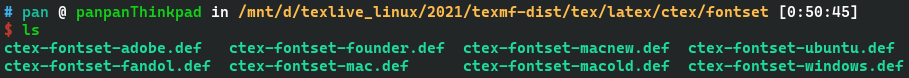
\includegraphics[width=\textwidth]{ctex_fontsets}
\end{figure}

\subsection{在ctex使用过程中的设置}

在引入\texttt{ctex}宏包的时候进行fontset的设置即可:\texttt{\\documentclass[fontset=windows]{ctexart}}
\end{document}
